%Hypothese 9: Durch die Einführung der 4-Tage Woche steigt die Bereitschaft zur Weiterbildung.
% Aktuell 1,2,3: 1000, h5: 790, h9: 380 Wörter

\chapter{Überprüfung der Hypothese 9}
\label{chap:hypothese9}

\section{Vorgehensweise}
Mit der Hypothese \gqq{Durch die Einführung der 4-Tage Woche steigt die Bereitschaft 
zur Weiterbildung} wird ein Fokus auf die 
Auswirkung der 4-Tage-Woche auf die Arbeitnehmenden gelegt. Auf Basis dieser Hypothese 
wurde in der Umfrage
die Frage \gqq{Würde eine 4-Tage-Woche Ihre Bereitschaft zur Weiterbildung in 
Ihrer Freizeit erhöhen?} an die Teilnehmenden gestellt.
Die Teilnehmenden konnten zwischen den Antwortmöglichkeiten \gqq{Ja}, \gqq{Eher Ja}, \gqq{Neutral}, 
\gqq{Eher Nein} und \gqq{Nein} wählen.

\paragraph*{Identifikation der relevanten Variablen}

Zu Beginn werden die unabhängigen, sowie die abhängige Variable identifiziert, welche für die 
Betrachung der Hypothese 9 relevant sind.

Die abhängige Variable beinhaltet die Daten zu der Antwort auf die Frage aus der Umfrage
\gqq{Würde eine 4-Tage-Woche Ihre Bereitschaft zur Weiterbildung in Ihrer Freizeit erhöhen?}.
Sie spiegelt direkt die Bereitschaft der Teilnehmenden zur Weiterbildung in ihrer Freizeit 
unter einer 4-Tage-Woche wider.

Für die Unabhängigen Variablen wurden die folgenden Variablen aus der Umfrage ausgewählt. 
Hier wird angenommen, dass diese Variablen einen Einfluss auf die Bereitschaft zur 
Weiterbildung der Teilnehmenden haben könnten.
\begin{itemize}
    \item Alter
    \item Geschlecht % vielleicht betrachten
    \item Kinder (Nominal)
    \item Vollzeit/Teilzeit
    % \item Führungsverantwortung
\end{itemize}


\paragraph*{Ausgewählte Analyseverfahren}

Für die Auswertung aller abgegebenen Antworten wird zuerst mit einer deskriptiven Analyse in Form eines Histogrammes
begonnen um die gesamte Meinung aller Teilnehmenden ohne Berücksichtigung der unabhängigen Variablen zu betrachten. 
Dieses ist mit einer Gaußschen Glockenkurve um den Mittelwert herum versehen, um zu betrachten, ob die Antworten 
normalverteilt sind. % warum ist das wichtig?
Hierzu werden ebenfalls der Modalwert (Modus), Median und Mittelwert der Antworten berechnet und angegeben,
um weitere Fakten über die Verteilung der Antworten zu erhalten. % Noch Standardabweichung?

Im Anschluss werden die bereits genannten unabhängigen Variablen durch Kreuztabellen betrachtet und
in passender Weise dargestellt, welche einen Einfluss auf die Bereitschaft zur Weiterbildung in der 
Freizeit unter einer 4-Tage-Woche haben könnten. 
Zusätzlich wird für die Variable des Alters eine Korrelationsanalyse durchgeführt, um zu prüfen, ob 
ein Zusammenhang zwischen diesem und der Bereitschaft besteht.



\section{Analyse}

In dem folgenden Histogramm \ref{fig:bereitschaft_weiterbildung_verteilung} wird die Verteilung 
der Antworten aller Teilnehmen auf die Frage \gqq{Würde eine 4-Tage-Woche Ihre Bereitschaft 
zur Weiterbildung in Ihrer Freizeit erhöhen?} betrachtet. Dabei konnten die Befragten zwischen den folgenden
Antwortmöglichkeiten wählen, welchen mit den dabei stehenden Nummern codiert worden sind:
 \gqq{Ja(1) }, \gqq{Eher Ja (2)}, \gqq{Neutral (3)}, \gqq{Eher Nein (4)} und \gqq{Nein (5)}

\begin{figure}[h]
    \centering
    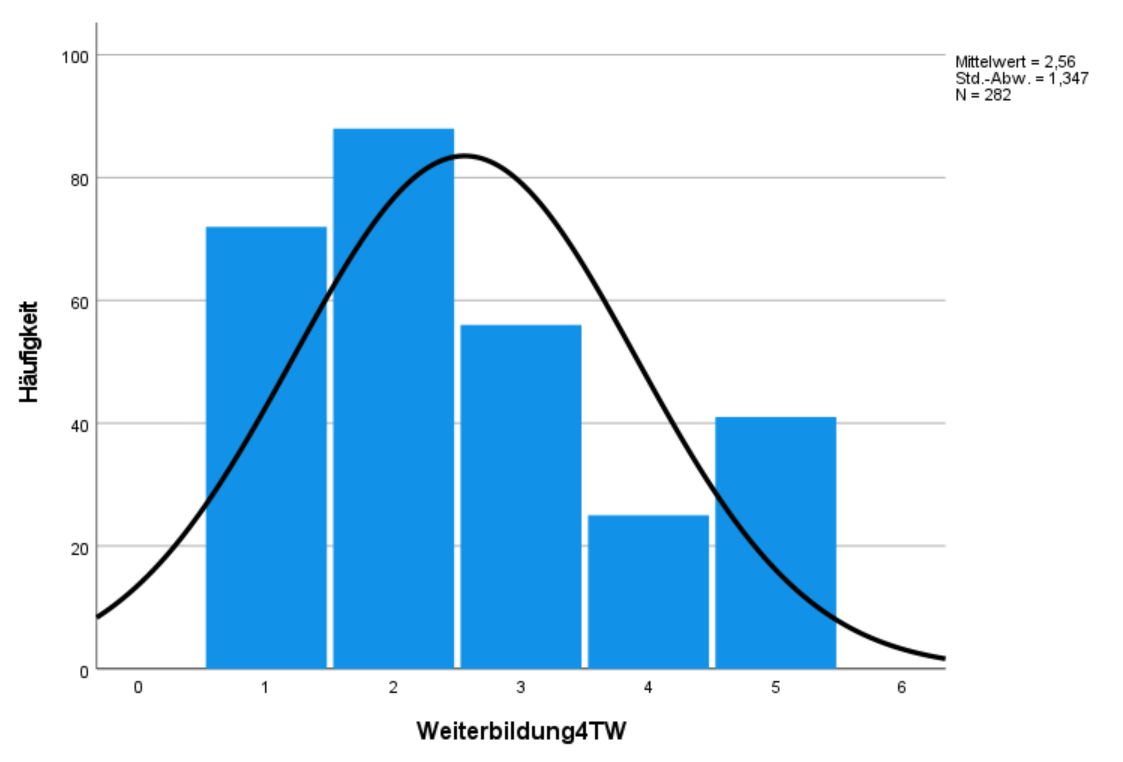
\includegraphics[width=0.7\textwidth]{04_Artefakte/01_Abbildungen/hypothese_9/histogramm_weiterbildung.png}
    \caption{Verteilung der Bereitschaft zur Weiterbildung in der Freizeit}
    \label{fig:bereitschaft_weiterbildung_verteilung}
\end{figure}

Aus dem Histogramm ist zu erkennen, dass die meisten Teilnehmenden eher 
eine Bereitschaft aufweisen sich in ihrer Freizeit weiterzubilden, 
wenn eine 4-Tage-Woche eingeführt wird.

Dies lässt ich auch anhand des Modalwertes (Modus) von 2 (Eher Ja) erkennen, welcher angibt, dass die
meisten Teilnehmenden die Bereitschaft zur Weiterbildung in ihrer Freizeit erhöhen würden.
Der Mittelwert von 2,56 und der Median von y zeigen ebenfalls auf, dass die Bereitschaft steigt.
Durch den Mittelwert ist allerdings zu erkennen, dass doch einige auch neutral oder negativ 
eingestellt sind.
% durch die Standardabweichung aufzeigen, dass die Meinung sich stärker unterscheidet?

\paragraph*{Alter}

Wie sich die Bereitschaft sich in der Freizeit weiterzubilden unter einer 4-Tage-Woche je nach Alter verändert,
kann in der Abbildung \ref*{fig:bereitschaft_weiterbildung_alter} betrachtet werden. 
Die Balken des Diagramms wurden nach Altersgruppen aufsteigend sortiert und normiert, um die Verhältnisse
der gegebenen Antworten zwischen den Altersgruppen besser vergleichen zu können.

\begin{figure}
    \centering
    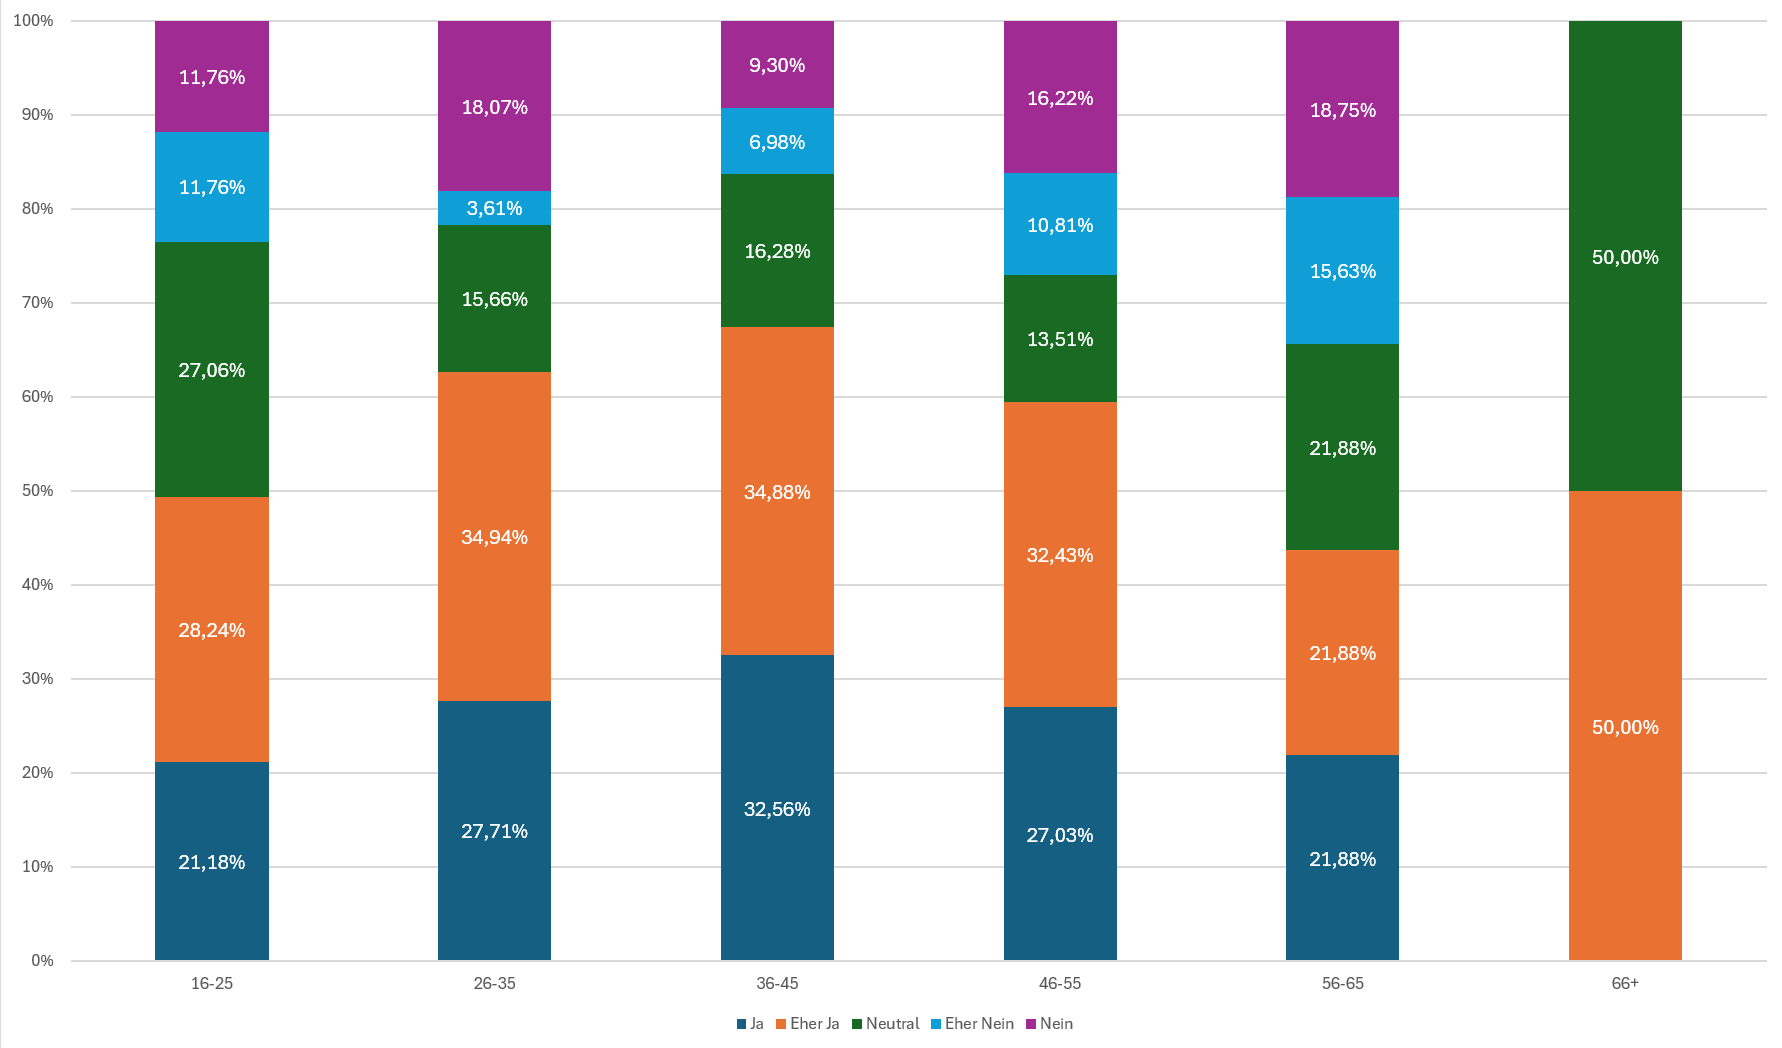
\includegraphics[width=0.7\textwidth]{04_Artefakte/01_Abbildungen/hypothese_9/weiterbildung_alter.png}
    \caption{Verteilung der Antworten zur Weiterbildung in der Freizeit unter Berücksichtigung des Alters}
    \label{fig:bereitschaft_weiterbildung_alter}
\end{figure}

Dabei fällt auf, dass bei einer Betrachtung von jung nach alt die Bereitschaft bis zur Altersgruppe von
36 bis 45 Jahren die Bereitschaft steigt. Ersichtlich durch die Zunahme der Antworten von Ja und Eher Ja.
In der Altersgruppe 36 bis 45 Jahren ist die Bereitschaft am höchsten und nimmt mit steigendem Alter
weiter hab. In der Altersgruppe von über 66 sind die Antworten zu vernachlässigen, da dort bloß
zwei Antworten durch die Umfrage eingegangen sind.

Für eine genauere Betrachtung wurde eine Korrelationsanalyse zwischen den beiden Variablen Alter 
und der Bereitschaft zu einer Weiterbildung durchgeführt. Hierbei wurde ein Korrelationskoeffizient 
von $-0,015$ ermittelt 
% \ref*{label:korrelation_bereitschaft_alter}, 
welcher darauf hinweist, dass kein Zusammenhang zwischen dem 
alter und der Bereitschaft zur Weiterbildung in der Freizeit unter einer 4-Tage-Woche besteht.
Erst ab einem Wert von $0,1$ oder $-0,1$ könnte von einer schwachen Korrelation gesprochen werden.


\paragraph*{Geschlecht}

Zum Einfluss des Geschlechts kann die Kreuztabelle \ref{tab:weiterbildung_geschlecht} betrachtet werden.
Hier ist zu erkennen, dass die Antworten zwischen Weiblich und Männlich relevant ähnlich sind. 
Bei genauerer Betrachtung fällt auf, dass männliche Teilnehmende eher negativ eingestellt sind, was durch
den größeren Anteil an Antworten von Eher Nein und Nein und dem kleineren Anteil an Ja Antworten
zu erkennen ist im Vergleich zu den weiblichen Teilnehmenden.


\begin{table}[h]
    \centering
    \begin{tabular}{cl|r|r|r|r|r|r|r|r|r}
    & & \multicolumn{8}{c|}{Geschlecht} \\
    & & \multicolumn{2}{c|}{Weiblich} & \multicolumn{2}{c|}{Männlich} & \multicolumn{2}{c|}{Divers} & \multicolumn{2}{c|}{Keine Angabe} \\ \hline
    & Ja        & 38 & 28,57\% & 33 & 22,76\% & 0 & 0\% & 1 & 100\% \\
    & Eher Ja   & 42 & 31,58\% & 45 & 31,03\% & 1 & 33,33\%   & 0 & 0\%   \\
    & Neutral   & 26 & 19,55\% & 30 & 20,69\% & 0 & 0\%   & 0 & 0\%   \\
    & Eher Nein & 10  & 7,52\%  & 14  & 9,66\%  & 1 & 33,33\%   & 0 & 0\%   \\
    \multirow{-5}{*}{\rotatebox[origin=c]{90}{Weiterbildung}} & Nein & 17 & 12,78\% & 23 & 15,86\% & 1 & 33,33\% & 0 & 0\%  \\ \hline
    &           & 133 & & 145 & & 3 & & 1 & & 282
    \end{tabular}
    \caption{Kreuztabelle der Meinung zu Weiterbildung in der Freizeit wenn eine 4-Tage-Woche vorliegt unter Berücksichtigung des Geschlechtes}
    \label{tab:weiterbildung_geschlecht}
\end{table}

\paragraph*{Kinder}



\begin{table}[h]
    \centering
    \begin{tabular}{cl|r|r|r|r|r}
    & & \multicolumn{4}{c|}{Kinder} \\
    & & \multicolumn{2}{c|}{Ja} & \multicolumn{2}{c|}{Nein}\\ \hline
    & Ja        & 27 & 25,96\% & 45 & 25,28\%  \\
    & Eher Ja   & 31 & 29,81\% & 57 & 32,02\%  \\
    & Neutral   & 21 & 20,19\% & 35 & 19,66\%   \\
    & Eher Nein & 8  & 7,69\%  & 17  & 9,55\%   \\
    \multirow{-5}{*}{\rotatebox[origin=c]{90}{Weiterbildung}} & Nein & 17 & 16,35\% & 24 & 13,48\%  \\ \hline
    &           & 104 & & 178 & & 282
    \end{tabular}
    \caption{Kreuztabelle der Meinung zu Weiterbildung in der Freizeit wenn eine 4-Tage-Woche vorliegt unter Berücksichtigung, ob die Befragte Person Kinder hat}
    \label{tab:weiterbildung_kinder}
\end{table}

\paragraph*{Vollzeit/Teilzeit}

Zu der unabhängigen Variable Vollzeit/Teilzeit war die Erwartung da, dass die Bereitschaft zur 
Weiterbildung unter einer 4-Tage-Woche bei Personen in Teilzeit niedriger wäre, da diese bereits
eine kürzere Arbeitszeit haben und somit mehr Freizeit zur Verfügung haben, um eine Weiterbildung
durchzuführen. Bei der Betrachtung der Kreuztabelle \ref{tab:weiterbildung_teilzeit_vollzeit} ist
zwar zu erkennen, dass Personen in Teilzeit eher negativ geantwortet haben, jedoch lässt sich
dies durch eine Korrelationsanalyse nicht bestätigen. Hierbei wurde ein Korrelationskoeffizient von $-0,042$
ermittelt, welcher darauf hinweist, dass kein Zusammenhang zwischen den beiden Variablen besteht.

\begin{table}[h]
    \centering
    \begin{tabular}{cl|r|r|r|r|r}
    & & \multicolumn{4}{c|}{Arbeitszeitmodell} \\
    & & \multicolumn{2}{c|}{Teilzeit} & \multicolumn{2}{c|}{Vollzeit}\\ \hline
    & Ja        & 13 & 22,41\% & 59 & 26,34\%  \\
    & Eher Ja   & 17 & 29,31\% & 71 & 31,70\%  \\
    & Neutral   & 15 & 25,86\% & 41 & 18,30\%   \\
    & Eher Nein & 3  & 5,17\%  & 22  & 9,82\%   \\
    \multirow{-5}{*}{\rotatebox[origin=c]{90}{Weiterbildung}} & Nein & 10 & 17,24\% & 31 & 13,84\%  \\ \hline
    &           & 58 & & 224 & & 282
    \end{tabular}
    \caption{Kreuztabelle der Meinung zu Weiterbildung in der Freizeit wenn eine 4-Tage-Woche vorliegt unter Berücksichtigung, ob die Befragte Person in Teilzeit oder Vollzeit arbeitet}
    \label{tab:weiterbildung_teilzeit_vollzeit}
\end{table}

% Korrelationskoeffizienten anschauen? Nur wenn Korrelationen zwischen den Variablen da ist,
% dann auch Regressionsanalyse durchführbar?

% 08 Teil 3

% 08 Teil 4
    % 1. Modellbildung - Notwenig? Nö, wegen SPSS?
    % 2. Berechnung der Regressionsfunktion - 2.5 (S8-97) Schrittweise?
    % 3. Test der Regressionsfunktion - Güte des Modells
    % 4. Test der Regressionskoeffizienten
    % 5. Test der Modellprämissen

\section{Ergebnis}

% Beantworten, ob die Hypothese abgelehnt oder beibehalten wird

% Annahme, da die Umfrage in dem näheren Umfeld von Personen durchgeführt wurde, die 
% Berufsbegleitend einen Master machen, kann vermutet werden, dass die Bereitschaft zur
% Weiterbildung in der Freizeit höher ist, als in der Allgemeinbevölkerung.
% Es besteht auch die Möglichkeit, dass Personen, die bereits eine Weiterbildung machen
% oder allgemein bereit sind eine Weiterbildung in ihrer Freizeit zu machen, nicht positiv 
% abgestimmt haben

% Schauen, ob die Hypothese abgelehnt oder beibehalten wird